\documentclass[9pt,toc=listof,paper=portrait,paper=24cm:17cm,mpinclude=true,captions=outerbeside,usegeometry=true,\jobname]{scrbook}
\usepackage{geometry} %[showframe]

\areaset{10cm}{18.8cm}
\setlength{\columnsep}{\marginparsep}   % the columnsep is used by KOMA captionbeside to separate the caption from the image

\savegeometry{defaultpage}

\usepackage{polyglossia}
\usepackage{csquotes}
\setmainlanguage{english}

\usepackage[table]{xcolor}
\usepackage{ragged2e}                           % RaggedLeft and RaggedRight commands (left align, right align)
\usepackage[hang]{footmisc}                     % hanging footnote, possible ragged but this introduces new breaks and consequently new pages
\usepackage{url}
\usepackage{hyperref}                           % references in PDF
\usepackage{cleveref}                           % provides \cref command
\usepackage{fnpct}                              % footnotes and punctuation make 1. -> .1
\usepackage{graphicx}                           % Include images
\usepackage{caption}
\usepackage{subcaption}                         % for subfigure
\usepackage{newfloat}                           % for \DeclareFloatingEnvironment
\usepackage[section]{placeins}                  % https://tex.stackexchange.com/questions/279/how-do-i-ensure-that-figures-appear-in-the-section-theyre-associated-with
\usepackage[natbib=true,backend=biber,style=alphabetic-verb]{biblatex}
\usepackage{mparhack}                           % For the right placement of marginpars. https://www.texfaq.org/FAQ-marginparside
\usepackage{xparse}                             % for environments
\usepackage[strict]{changepage}                 % for wider then the typearea
\usepackage{shorttoc}
\usepackage{calc}                               % for geometry calculations

\setlength{\footnotemargin}{\parindent}

% draw frame around the complete page
%\usepackage{eso-pic}
%\AddToShipoutPictureBG{\begin{tikzpicture}[overlay,remember picture]
% \draw (current page.south west) rectangle (current page.north east);
%\end{tikzpicture}}

%% Configure Bibliography
\addbibresource{references.bib}
\DeclareRefcontext{web}{labelprefix=Web:}

\setsansfont{Open Sans}[
UprightFont = {* Condensed Light},
ItalicFont = {* Condensed Light Italic},
BoldFont = {* Condensed Bold},
]

\setkomafont{pageheadfoot}{\large\sffamily}
\setkomafont{pagenumber}{\large\sffamily}

% For more caption customization
% https://tex.stackexchange.com/a/318175/11820

\captionsetup[listing]{name={Listing}}

\captionsetup{format=plain, labelfont={bf}, font=footnotesize}
% , singlelinecheck=off

% \begin{disfigure}[short title]{long title}{label}
%   content
% \end{disfigure}
% Stared for wide figures
\NewDocumentEnvironment{disenv}{ o m m }
{
  \checkoddpage
  \ifoddpage
    %odd
    \captionsetup{justification=RaggedRight}
  \else
    %even
    \captionsetup{justification=RaggedLeft}
  \fi
  \begin{captionbeside}%
  [\IfValueTF{#1}{#1}{#2}]% short title
  {#2\label{#3}}
  [o]% caption on the outer document side
  [\dimexpr\textwidth+\marginparwidth+\marginparsep\relax]% enlarge the used width
  [0pt]*% align with the inner margin
  \begin{minipage}[b]{\textwidth}
}
{
  \end{minipage}
  \end{captionbeside}
}
\NewDocumentEnvironment{disenv*}{ o m m }
{
  \begin{adjustwidth*}{}{\dimexpr-\marginparwidth+\marginparsep\relax}
%  \begin{minipage}[b]{\dimexpr\textwidth+\marginparwidth+\marginparsep\relax}
}
{
  \end{adjustwidth*}
  \caption[\IfValueTF{#1}{#1}{#2}]{#2}
  \label{#3}
}

\NewDocumentEnvironment{disfigure}{ o m m }
{
  \begin{figure}[htbp]
    \begin{disenv}[#1]{#2}{#3}
}
{
    \end{disenv}
  \end{figure}
}
\NewDocumentEnvironment{disfigure*}{ o m m }
{
  \begin{figure}[htbp]
    \begin{disenv*}[#1]{#2}{#3}
}
{
    \end{disenv*}
  \end{figure}
}

\NewDocumentEnvironment{dislisting}{ o m m }
{
  \begin{listing}[htbp]
    \begin{disenv}[#1]{#2}{#3}
}
{
    \end{disenv}
  \end{listing}
}
\NewDocumentEnvironment{dislisting*}{ o m m }
{
  \begin{listing}[htbp]
    \begin{disenv*}[#1]{#2}{#3}
}
{
    \end{disenv*}
  \end{listing}
}

\NewDocumentEnvironment{distable}{ o m m }
{
  \begin{table}[htbp]
    \begin{disenv}[#1]{#2}{#3}
}
{
    \end{disenv}
  \end{table}
}
\NewDocumentEnvironment{distable*}{ o m m }
{
  \begin{table}[htbp]
    \begin{disenv*}[#1]{#2}{#3}
}
{
    \end{disenv*}
  \end{table}
}

\newcommand{\chapcite}[1]{%
  \citeauthor{#1}: \citetitle{#1} \cite{#1}%
}
\newcommand{\chapterref}[1]{%
  \marginpar{%
    \checkoddpage%
    \ifoddpage%
      %odd
      \RaggedRight%
    \else%
      %even
      \RaggedLeft%
    \fi%
    \footnotesize%
    \vspace{.44\baselineskip}
    \textcolor{black!80}{The results presented in this chapter were first published in #1}\par%
  }
}
\newcommand{\partsecref}[1]{%
  \marginpar{%
    \checkoddpage%
    \ifoddpage%
      %odd
      \RaggedRight%
    \else%
      %even
      \RaggedLeft%
    \fi%
    \footnotesize%
    \vspace{.44\baselineskip}
    \textcolor{black!80}{Parts of this section were first published in #1}\par%
  }
}


% Just a helper method for length
% FROM https://tex.stackexchange.com/a/239496/11820
\makeatletter
\def\convertto#1#2{\strip@pt\dimexpr #2*65536/\number\dimexpr 1#1}
\makeatother

% avoid footnote break
% https://tex.stackexchange.com/questions/68229/unwanted-pagebreak-in-footnote
\interfootnotelinepenalty=10000
% Avoid overfull hboxes
\emergencystretch=1em

% Highlight overfull hboxes
%\overfullrule=1mm

% Avoid Hurenkinder and so on
\clubpenalty = 10000
\widowpenalty = 10000
\displaywidowpenalty = 10000

\usepackage{afterpage}
\newcommand\blankpage{%
\null
\thispagestyle{empty}%
%\addtocounter{page}{-1}%
\newpage}

%%% START OF CONTENT

\title{The Dissertation Title}

\author{Your Name}
\date{2024-06-07}


\makeatletter
\newcommand{\myTitle}{\@title}
\newcommand{\mySubtitle}{Some Subtitle}
\newcommand{\myDocumentType}{Dissertation}
\newcommand{\myName}{\@author}
\newcommand{\myReihe}{Publikationen in der Informatik | Band X}
\makeatother

\hypersetup{
  pdfauthor=\myName,
  pdftitle=\myTitle,
}

%\recalctypearea
\begin{document}

\pagestyle{empty}
% Schmutztitel
\begin{titlepage}
\begin{flushright}
\strut

\vspace{3cm}
{\Large\myName}

\vspace{1cm}

{\sffamily\huge\textbf{\myTitle}\par}
\vspace{.5cm}
{\sffamily\Large\mySubtitle}

\vspace{1cm}
{\Large\myDocumentType}

\vfill
{\Large\myReihe}
\end{flushright}
\end{titlepage}

% Frontispiz
%\clearpage
% Titelblatt
%\clearpage

% Impressum

\begin{flushleft}
  \small
\strut


%paperwidth=\the\paperwidth\ \convertto{mm}{\the\paperwidth} mm\\
%paperheight=\the\paperheight\ \convertto{mm}{\the\paperheight} mm\\
%textwidth=\the\textwidth\ \convertto{mm}{\the\textwidth} mm\\
%textheight=\the\textheight\ \convertto{mm}{\the\textheight} mm\\
%marginparwidth=\the\marginparwidth\ \convertto{mm}{\the\marginparwidth} mm\\
%marginparsep=\the\marginparsep\ \convertto{mm}{\the\marginparsep} mm\\
%hoffset=\the\hoffset\\
%oddsidemargin=\the\oddsidemargin\\
%voffset=\the\voffset\\
%headsep=\the\headsep\\
%headheight=\the\headheight\\
%topmargin=\the\topmargin\\
%
%\newlength{\baselinehead} \setlength{\baselinehead}{1in+\voffset+\topmargin+\headheight}
%\newlength{\randinnen}    \setlength{\randinnen}{1in+\hoffset+\oddsidemargin}
%\newlength{\randoben}     \setlength{\randoben}{\baselinehead+\headsep}
%\newlength{\randunten}    \setlength{\randunten}{\paperheight-\randoben-\textheight}
%\newlength{\randaussen}   \setlength{\randaussen}{\paperwidth-\randinnen-\textwidth}
%\newlength{\randaussenmargin}   \setlength{\randaussenmargin}{\paperwidth-\randinnen-\textwidth-\marginparsep-\marginparwidth}
%
%innen=\the\randinnen\ \convertto{mm}{\the\randinnen} mm\\
%oben=\the\randoben\ \convertto{mm}{\the\randoben} mm\\
%unten=\the\randunten\ \convertto{mm}{\the\randunten} mm\\
%aussen=\the\randaussen\ \convertto{mm}{\the\randaussen} mm\\
%aussen mit margin=\the\randaussenmargin\ \convertto{mm}{\the\randaussenmargin} mm\\
%baselinehead=\the\baselinehead\ \convertto{mm}{\the\baselinehead} mm\\

\vfill

\textbf{Autor}

\myName\\
WebID: \url{https://natanael.arndt.xyz/#i}, \url{http://aksw.org/NatanaelArndt}\\
ORCID: \url{https://orcid.org/0000-0002-8130-8677}\\
DBpedia Global ID: \url{https://global.dbpedia.org/id/CHPU2}

\begin{FlushLeft}
\textbf{Bibliografische Information der Deutschen Nationalbibliothek}

Bibliografische Information der Deutschen Nationalbibliothek: Die Deutsche Nationalbibliothek verzeichnet diese Publikation in der Deutschen Nationalbibliografie; detaillierte bibliografische Daten sind im Internet über\linebreak \url{http://dnb.dnb.de} abrufbar.

\vspace{1em}

Der Text dieses Werks ist unter der Creative-Commons-Lizenz\linebreak CC BY-NC 4.0 International veröffentlicht. Den Vertragstext der Lizenz finden Sie unter \url{https://creativecommons.org/licenses/by-nc/4.0/}.
Die Abbildungen sind von dieser Lizenz ausgenommen, hier liegt das Urheberrecht beim jeweiligen Rechteinhaber.
\marginpar{\raggedleft\includegraphics[]{images/cc-by-nc_icon}}
Wenn sie darüber hinausgehende Rechte benötigen wenden sie sich bitte an den Autor.
\end{FlushLeft}

\marginpar{\raggedleft\vspace{.01cm}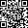
\includegraphics[width=.4\marginparwidth]{images/doi}}

\textbf{Die Online-Version dieser Publikation ist abrufbar unter}

\url{https://doi.org/10.33968/9783966270205-00}

\vspace{1em}

© 2023 \myName

\vspace{1em}

\textbf{Herausgeber der Reihe}

Institut für Informatik an der\linebreak Hochschule für Technik, Wirtschaft und Kultur Leipzig

\vspace{1em}

\textbf{Verlag}

Open-Access-Hochschulverlag\\
Hochschule für Technik, Wirtschaft und Kultur Leipzig\\
Karl-Liebknecht-Str. 132, 04277 Leipzig, Deutschland

\vspace{1em}

Herstellung: BoD – Books on Demand, Norderstedt\\
Cover: 

\vspace{1em}

ISBN (Softcover) 978-3-96627-019-9\\
ISBN (ePub) 978-3-96627-021-2\\
ISBN (PDF) 978-3-96627-020-5
\end{flushleft}
\clearpage

%\pagestyle{headings}
%\setcounter{tocdepth}{0}
\shorttableofcontents{Contents}{0}
\vfill
\clearpage


\pagestyle{headings}

\newgeometry{%
textwidth=\textwidth+\marginparwidth-\marginparsep,
textheight=\textheight,
top=1in+\voffset+\topmargin+\headheight+\headsep,
inner=1in+\hoffset+\oddsidemargin,
marginparsep=\marginparsep,
marginparwidth=\marginparsep,
}
\savegeometry{widepage}

\section*{Vorwort A}
\addcontentsline{toc}{chapter}{Preface by A}

\vspace{1cm}

\noindent
Who

\clearpage

\section*{Preface A}


\vspace{1cm}

\noindent
Who

\clearpage
\pagestyle{empty}
\null
\clearpage
\pagestyle{headings}

\section*{Preface B}
\addcontentsline{toc}{chapter}{Preface by B}


\vspace{1cm}

\noindent
Who

\clearpage

\pagestyle{empty}
\restoregeometry
\pagestyle{headings}

\section*{Zusammenfassung}
%\begin{german}
Ziel dieser Arbeit ist es, die Entwicklung von RDF-Wissensbasen in verteilten kollaborativen Szenarien zu unterstützen.
In dieser Arbeit wird eine neue Methodik für verteiltes kollaboratives Knowledge Engineering – „Quit“ – vorgestellt.
Sie geht davon aus, dass es notwendig ist, während des gesamten Kooperationsprozesses Dissens auszudrücken und individuelle Arbeitsbereiche für jeden Mitarbeiter bereitzustellen.
Der Ansatz ist von der Git-Methodik zum kooperativen Software Engineering inspiriert und basiert auf dieser.
Die Analyse des Standes der Technik zeigt, dass kein System die Git-Methodik konsequent auf das Knowledge Engineering überträgt.
Die Hauptmerkmale der Quit-Methodik sind unabhängige Arbeitsbereiche für jeden Benutzer und ein gemeinsamer verteilter Arbeitsbereich für die Zusammenarbeit.
Während des gesamten Kollaborationsprozesses spielt die Data-Provenance eine wichtige Rolle.
Zur Unterstützung der Methodik ist der Quit-Stack als eine Sammlung von Microservices implementiert, die es ermöglichen, die Semantic-Web-Datenstruktur und Standardschnittstellen in den verteilten Kollaborationsprozess zu integrieren.
Zur Ergänzung der verteilten Datenerstellung werden geeignete Methoden zur Unterstützung des Datenverwaltungsprozesses erforscht.
Diese Managementprozesse sind insbesondere die Erstellung und das Bearbeiten von Daten sowie die Publikation und Exploration von Daten.
Die Anwendung der Methodik wird in verschiedenen Anwendungsfällen für die verteilte Zusammenarbeit an Organisationsdaten und an Forschungsdaten gezeigt.
Weiterhin wird die Implementierung quantitativ mit ähnlichen Arbeiten verglichen.
Abschließend lässt sich feststellen, dass der konsequente Ansatz der Quit-Methodik ein breites Spektrum von Szenarien zum verteilten Knowledge Engineering im Semantic Web ermöglicht.
%\end{german}

\clearpage
%\pagebreak

\section*{Abstract}
The aim of this thesis is to support the development of RDF knowledge bases in a distributed collaborative setup.
In this thesis a new methodology for distributed collaborative knowledge engineering – called Quit – is presented.
It follows the premise that it is necessity to express dissent throughout a collaboration process and to provide individual workspaces for each collaborator.
The approach is inspired by and based on the Git methodology for collaboration in software engineering.
The state of the art analysis shows that no system is consequently transferring the Git methodology to knowledge engineering.
The key features of the Quit methodology are independent workspaces for each user and a shared distributed workspace for the collaboration.
Throughout the whole collaboration process data provenance plays an important role.
To support the methodology the Quit Stack is implemented as a collection of microservices, that allow to integrate the Semantic Web data structure and standard interfaces with the distributed collaborative process.
To complement the distributed data authoring, appropriate methods to support the data management process are researched.
These management processes are in particular the creation and authoring of data as well as the publication and exploration of data.
The application of the methodology is shown in various use cases for the distributed collaboration on organizational data and on research data.
Further, the implementation is quantitatively compared to the related work.
Finally, it can be concluded that the consequent approach followed by the Quit methodology enables a wide range of distributed Semantic Web knowledge engineering scenarios.

%The methodology supports \emph{dissent} during the collaboration process and \emph{asynchrony} of individual workspaces on the distributed workspace.
%To achieve this support atomic evolution operations are identified and stored in a canonical representation.
%Based on this representation various methods are presented to \emph{synchronize} the workspaces, \emph{reconcile} diverged states of the workspaces, and track \emph{provenance} information during the collaborative process.

%The relevant preliminaries are shown

%It has the ability to handle dissent as a process of collaboration to reach consensus.
%The results of the collaborative process can be published to a wide audience
%The methodology is flexible in its adaption to new domains by providing the possibility to build domain-specific creating and authoring interfaces as well as domain-specific exploration interfaces.

\clearpage

\section*{Acknowledgements}
The excitement for using the Semantic Web to organize data and communicate using the RDF data format was brought to me by the Agile Knowledge Engineering and Semantic Web (AKSW) work group at the Chair of Business Information Systems (BIS) at the Leipzig University and the Institute for Applied Informatics (InfAI).
I want to thank the whole AKSW group as well es all students who supported our development and research.
Among everyone there are some people who play a special role, Dr. Sebastian Tramp brought me into the whole topic, Norman Radtke accompanied me on my way through the Semantic Web from beginning until now, Dr. Michael Martin made so many things possible and keeps things running, and Simon Bin and many more invest much time and patience to keep our infrastructure running.
I want to thank Prof. Dr. Klaus-Peter Fähnrich who gave us all the freedom for development and research.
I want to thank Simone Angermann for keeping his spirit alive.
I want to thank Prof. Dr. Sören Auer, he founded the AKSW group and constantly brings people to work together, he always gives me good advise.
Especially, I want to thank my supervisor Prof. Dr. Thomas Riechert, he is there in the right moments and helps out with the right things, I'm grateful to work with him.

Besides the people immediately around me there are so many more people in the Semantic Web community, who I could meet during conferences from whom I received feedback on my thoughts and work.
In the community I especially want to thank Dr. Jeremy Debattista, Dr. Jürgen Umbrich, and Dr. Javier David Fernández Garcia for the organization of the MEPDaW 2017 and the organization of the subsequent shepherding program.
I want to thank Prof. Dr. Olaf Hartig for his time and patience in being my shepherd.
I want to thank the unknown reviewers of my papers for their critical and helpful reviews.

A lot of my work was done during research projects funded by the European Commission from the European Regional Development Fund (ERDF), the German Federal Ministry of Education and Research (BMBF), and the Federal Ministry for Economic Affairs and Energy (BMWi).
I also received a scholarship from the Science Foundation Ireland (SFI) for my time in Galway and I was supported by a travel grant from the German Academic Exchange Service (DAAD).

My family and friends always support me, cook for me, host me, and give me the freedom I need.
They had to endure my absence and motivated me to finish this thesis.
I want to thank Dorothea, Timotheus, Tamar, Jonathan, Rafael, Katharina, Rahel, Florian, Rebekka, Tabea, Norman, Markus, Claudius, Sebastian, Franziska, Sebastian, Markus, and Barbara.
They give me valuable remarks, ask important questions, shift my focus to the important things in life, and supported me in proofreading.
My wife and my daughter had to bear with me working at the weekend and during holidays but still I receive special support and so much more from Tracy and Hodaja, thank you.

\clearpage
\renewcommand\pagemark{\usekomafont{pagenumber}\thepage}
\setcounter{tocdepth}{1}
\tableofcontents


%\tableofcontents

\chapter*{Preface}

% Knowledge Graphs over Large Data Sources: Construction, Exploration and Analytics
\section{Introduction}

Data integration, the process to provide a uniform view over data from multiple sources in various formats, is among the top challenges in modern information societies and gave rise to a vast amount of research over the past decades. The Semantic Web proposes a uniform and extensible Web-scale model for data with well defined semantics. This not only enables human and software agents to access data in a machine readable way, but it also allows them to reason about the data. In the Semantic Web, datasets are modeled as graphs.
Datasets can be easily combined into a larger one which results in a larger graph.
The term \textit{Knowledge Graph} (KG) has been established because such graphs can capture and connect (meta-)information
from virtually arbitrary domains\footnote{The work focuses on Semantic Web Knowledge Graphs in constrast to Property Graphs.}.
The essential technologies are the Resource Description Framework (RDF) which specifies the graph based data model.
Databases that can store RDF data are referred to as RDF stores\footnote{Other common names are \textit{triple store} and \textit{quad store} referring to more in-depth aspects of RDF stores.}.
The standard language to query and update RDF stores is called \textit{SPARQL}\footnote{SPARQL is a recursive acronym for \textit{SPARQL Protocol and RDF Query Language}. Sometimes the acronym SPARUL is used to specifically refer to the Update Language. Note, that the situation is similar to the \textit{Structured Query Language} (SQL) which subsumes the sub-languages for querying, updating and data definition.}.

\subsection{Motivation}

The motivation for this thesis touches three related fields: The construction of KGs, the exploration of KGs and the benchmarking KG setups.

The promise of a Knowledge Graph is that operations on the uniform data layer become sufficiently simple such that it offsets the resource investment into that graph's construction. An important feat of knowledge graphs is that they enable human and machine agents to explore the data of \textit{virtually any domain} via defined interfaces and protocols, i.e. SPARQL. Over the years, the conceptual approach to building knowledge graphs has to large parts transitioned from art to engineering: Best practices for common design challenges (e.g. IRI, vocabulary, ontology) have been devised and mapping languages were developed to transform non-RDF data to RDF. Yet, in practice one encounters many difficulties: Knowledge Graph Construction (KGC) tools differ greatly w.r.t. performance, scalability, supported mapping languages, extensibility (e.g. user defined functions), and supported optimizations. The combination of KGC tooling with Big Data technologies is thus an interesting field to explore.

Once a constructed KG is accessible via SPARQL, the next challenge is how to make it explorable, such that an agent can access and identify relevant subsets of the data. Faceted search is an exploratory search technique that allows narrowing down sets of information items by applying constraints over their properties, whereas facets correspond to properties of these items. Faceted search can be used directly to explore the (partial) output of a KC process and thus has direct application for rapid-prototyping. Furthermore, complementary approaches, such as data summarizations, may be computed ad-hoc for only the narrowed down set of items. The RDF model exhibits several traits that seemingly make it a natural foundation for faceted search: all information items are represented as RDF resources, property values typically already correspond to meaningful semantic classifications, and with SPARQL there is a standard language for uniformly querying instance and schema information. However, although faceted search is ubiquitous today, it is typically not performed on the RDF model directly. Two major sources of concern are the complexity of query generation and the query performance.

And finally, while RDF stores provide standard SPARQL endpoints, there are substantial differences between the different systems. The basic effect is that SPARQL queries that run well on one system may run poorly on another and vice versa. While there are standard benchmarks for RDF databases, there is a lack of systematic analysis of how triple stores perform for different categories of *real-world* SPARQL queries.

\subsection{Goals}

The overall goal of this thesis is to ease both the construction Knowledge Graphs from heterogeneous data sources, facilitate their exploration and provide the means to evaluate KG setups.

For the KG construction, the goal is to leverage Big Data approaches for parallelization and integrating (SPARQL) extensions that simplify tackling certain integration problems in order to produce high quality data fast.

Exploration of knowledge graphs is essential for spotting mistakes introduced by the construction process as well as assessing its fitness for use. In general, faceted search, as a type of exploratory search, is a proven approach to explore collections of information items. However, there are many challenges in adopting this paradigm to KGs. The first goal is to devise a model for faceted search that supports traversal along the properties of information items in a KG. The subsequent goal is to devise how to generate appropriate SPARQL queries from that model.

In order to evaluate KG setups on real wold queries (rather than synthetic ones), a framework needs to be devised that allows for categorization of SPARQL queries based on their features and supports detailed query execution reports, such as intermediate result set sizes and execution times.

In general, for the sake of reproducibility, all relevant code should be published as Open Source software.

\subsection{Research Questions}

This thesis contributes to the following fundamental challenges in the Semantic Web that build on one another are:
(1) The efficient construction of large-scale knowledge graphs, both by means of data materialization and virtualization.
(2) The exploration of information contained in a knowledge graph as a prerequisite to assess fitness for use.
Thereby approaches for modeling and indexing the metadata need to be considered.
(3) The analysis of SPARQL query performance against RDF stores in order to detect limitations, feature- or performance-wise, on contemporary triple stores as a basis for improvement.

The research question for each part-challenge are as follows:

\begin{itemize}
\item Large-Scale KG Construction
  \begin{itemize}
    \item How well does visualization of (spatial) relational databases perform and what are strengths and limitations?
    \item To what extent can we leverage (map-reduced-based) Big Data technology, such as Apache Spark?
    \item How can we leverage either approach to create summarization meta data from large RDF datasets, such as VoID descriptions?
  \end{itemize}
\item KG Exploration:
  \begin{itemize}
  \item As Faceted Search is an established means for exploring catalogs, such as products and images, by means of restricting a result set to those items that match a set of constraints. The question is to what extent can the Faceted Search paradigm be adapted to operate on KGs via SPARQL.  Also, operations known from Business Intelligence systems and Data Cubes (e.g. drill down) are very relevant topics that need to be investigated.
  \item What are feature and/or performance limitations of the SPARQL queries that correspond to Faceted Search information needs on real-world RDF stores?
  \end{itemize}
\item RDF Store Analysis: The aim of this part is to generalize assessment of query performance to arbitrary real-world queries (not limited to faceted search ones).
  \begin{itemize}
  \item How to devise a model that captures detailed aspects of the execution of arbitrary SPARQL query queries?
  \item A goal is to collect SPARQL query logs from real-world SPARQL endpoints. How to process such logs efficiently?
  \end{itemize}
\end{itemize}

\subsection{Methodological Approach}

In regard to knowledge graph construction, the approach is to systematically review existing approaches and to devise a novel solution based on the map-reduce paradigm using a Big Data framework such as Apache Spark. A scientific evaluation will compare this novel approach with existing ones w.r.t. performance, scalability and feature set.

For faceted search there exist models for varying level of complexity to capture information needs. An review will be done with the goal to devise a model that takes the characteristics of KGs into account and which can operate on standard SPARQL endpoints. Hence, requirements for faceted search on knowledge graphs need to be devised, most likely based on (hypothetical) UI interactions. The focus is here on the query model and query generation rather than a concrete UI design. On this basis, aspects such as the representation of constraints and the query generation need to be derived. A foreseeable challenge in this regard will be to find a trade off between complexity and expressiveness.

For the KG setup evaluation, the approach is to collect real world query log files from popular SPARQL endpoint hosts, such as DBpedia. A system will be designed and implemented that first extracts static information from SPARQL queries. Then the queries will be decomposed into relevant "fragments", such as basic graph patterns, and the query and its fragments will be benchmarked individually against a configurable RDF store. On this basis, it is expected that scientific insights can be obtained, such as related to the frequency of sparse joins and the use of standard SPARQL features and custom query extensions.

An RDF model needs to be devised that supports the representation of information from static query analysis and connecting it with the obtained runtime information (such as intermediate result set sizes, execution times, counts of distinct values). It is expected that the implementation of this analysis framework can benefit from the experience gathered by the efforts that combine knowledge graph construction with Big Data. The faceted search approach should make it possible to browse and explore reasonably sized subsets of the produced benchmark data.


\chapter*{Acknowledgements}

\todo{Reference all the projects across the papers}



\chapter*{Methodology}

% The Methodology
\chapterref{%
\chapcite{arndt-n-2017--decentralized}; % ICWE
\chapcite{arndt-n-2018--jws}; % JWS
and \chapcite{arndt-n-2019--qeicc}.% % QEICC
}

This chapter provides an overview on the  methodology.




\end{document}
